\section{Computational Results}

We simulated performance of our algorithms on random graphs generated by the graph models we outlined. The following graphs show that the lower bound we calculated for the expected performance of the sampling algorithm accurately captures the behavior of the sampling algorithm when $a=1$. Indeed, the inequality we used is an accurate approximation of the true expectation, up to lower order terms. The random sampling algorithm does well, both when $c$ is low and high, but falters when $ck=1$. The greedy algorithm performs better than the random sampling algorithm in all cases, but its advantage vanishes $c$ gets larger. In all the graphs below, the red line indicates the performance of the greedy algorithm and the blue line indicates the performance of the random sampling algorithm.

\begin{figure}[h]
\centering
\begin{minipage}[h]{0.45\textwidth}
\centering
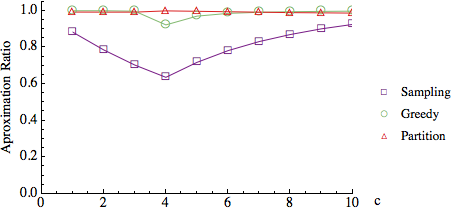
\includegraphics[width=0.8\textwidth]{images/l=25000,r=100000_Greedy_vs_Naive.png}
\caption{Approximation ratios when |L|=25k, |R|=100k, d=20, a=1}
\end{minipage}
\hspace{0.2cm}
\begin{minipage}[h]{0.45\textwidth}
\centering
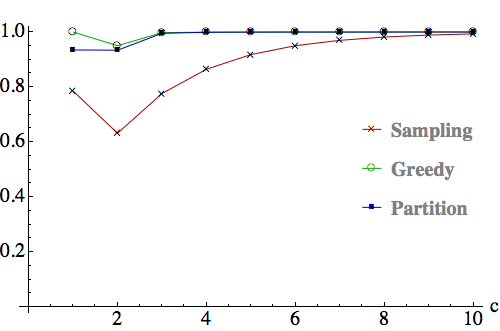
\includegraphics[width=0.8\textwidth]{images/l=50000,r=100000_Greedy_vs_Naive.png}
\caption{Approximation ratios when |L|=50k, |R|=100k, d=20, a=1}
\end{minipage}
\end{figure}

In contrast to the case when $a=1$, the sampling algorithm performs much more poorly when $a>1$. In such cases, the sampling algorithm performs well only when $c$ is large. The greedy algorithm continues to give solutions that are nearly optimal, regardless of the settings of $c$ and $a$. Therefore, our simulations suggest that in all cases, the greedy algorithm is a suitable and simple replacement for solving the problem to optimality.

\begin{figure}[h]
\centering
\begin{minipage}[h]{0.45\textwidth}
\centering
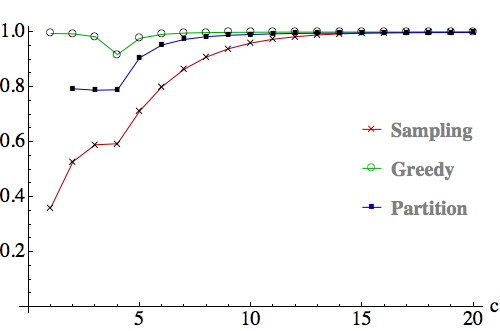
\includegraphics[width=0.8\textwidth]{images/l=50000,r=100000,a=2_Greedy_vs_Naive.png}
\caption{Approximation ratios when |L|=50k, |R|=100k, d=20, a=2}
\end{minipage}
\hspace{0.2cm}
\begin{minipage}[h]{0.45\textwidth}
\centering
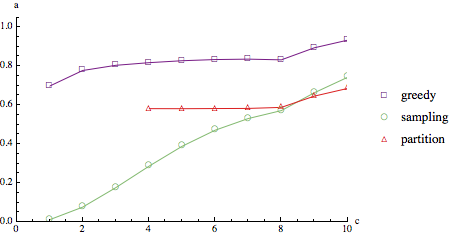
\includegraphics[width=0.8\textwidth]{images/l=50000,r=100000,a=4_Greedy_vs_Naive.png}
\caption{Approximation ratios when |L|=50k, |R|=100k, d=20, a=4}
\end{minipage}
\end{figure}